\documentclass[DM,lsstdraft,authoryear,toc]{lsstdoc}
% lsstdoc documentation: https://lsst-texmf.lsst.io/lsstdoc.html

% Package imports go here.
\usepackage{booktabs}
\usepackage{xspace}
\usepackage{hyperref}
\usepackage{graphicx}

% Local commands go here.
\newcommand{\opsim}{\texttt{OpSim}\xspace}
\newcommand{\socs}{\texttt{SOCS}\xspace}
\newcommand{\sched}{\texttt{Scheduler}\xspace}
\newcommand{\simsky}{\texttt{sims\_skybrightness}\xspace}
\newcommand{\magasq}{magnitude/arcsecond$^{2}$\xspace}

% To add a short-form title:
% \title[Short title]{Title}
\title{A New Baseline Operations Simulation with Dome Crawl}

% Optional subtitle
% \setDocSubtitle{A subtitle}

\author{%
Owen Boberg,
Lynne Jones,
Tiago Ribeiro, \\
\v{Z}eljko Ivezi\'{c}}

\setDocRef{baseline-opsim}

\date{\today}

% Optional: name of the document's curator
% \setDocCurator{The Curator of this Document}

\setDocAbstract{%
We present an update to the recently released baseline simulated survey (baseline2018a), created using \opsim v4.1.2.2.
The updated simulation we present here does not change the observing strategy used in baseline2018a (i.e. same hour angle bonus values, survey footprint, etc.),
but does implement changes to the Observatory Model used by \opsim. Specifically, the new simulations use a crawling
dome model and a longer closed loop (CL) active optics delay. We find that implementing a crawling dome model increases the total number of visits
over 10 year by $3\%$ and the longer CL delay does not significantly decrease the number of visits. }

% Change history defined here.
% Order: oldest first.
% Fields: VERSION, DATE, DESCRIPTION, OWNER NAME.
% See LPM-51 for version number policy.
\setDocChangeRecord{%
  \addtohist{1}{YYY-MM-DD}{Unreleased.}{Owen Boberg}
}

\begin{document}

% Create the title page.
% Table of contents is added automatically with the "toc" class option.
\maketitle

\section{Overview}

The following are the minor changes made to \opsim v4 to produce the new baseline presented in this document:

\begin{itemize}
\item Added capability to use a crawling dome model to reduce the dome slew time in azimuth.
\item The closed loop (CL) active optics delay was increased from 20 seconds to 36 seconds.
This increase was proposed, and accepted, by telescope and site to the LSST project management CCB.
\item The sims\_skybrightness\_pre data were generated using HealPix skymaps instead of OpSim fields.
\end{itemize}

Here we present a list of simulated surveys (see Table \ref{tab:runlist}) created using \opsim v4 to understand
the effects of enabling dome crawl and extending the CL correction delay. Each of these runs uses the same Hour
Angle bonus and Hour Angle max values used in baseline2018a, and the only differences in their configurations is the
addition of dome crawl and the longer CL correction delay. We first generated a simulation with just the new dome crawl model
enabled, pontus\_2003, to understand its effect in isolation. The second new simulation, kraken\_2026, has both the
dome crawl model enabled and the longer CL correction delay. We recommend adopting kraken\_2026 as the a replacement
for baseline2018a.

\begin{table}[htp]
\caption{Short list of simulated surveys illustrating \opsim changes.}
\begin{center}
\begin{tabular}{ l | l | l }
\toprule
\opsim Run & Version & Summary \\
\midrule
baseline2018a &   &  No dome crawl, CL delay 20 seconds\\
pontus\_2003  &   &  dome crawl, CL delay 20 seconds\\
kraken\_2026  &   &  dome crawl, CL delay 36 seconds\\
\bottomrule
\end{tabular}
\end{center}
\label{tab:runlist}
\end{table}

\section{Crawling dome model}

In real-time operation, dome crawling (or dome creep) takes advantage of the slightly oversized dome slit to reposition the dome in advance.
The idea derives from the fact that the dome is slower than the telescope, which could cause an important loss of efficiency if not treated properly.
At the same time, the LSST dome also operates as a light baffle, so there's some constraint to how large it can be. To mitigate the slew problem
without compromising light baffling, the dome slit was designed to accommodate a telescope slew of 4 degrees in azimuth without the need to
move the dome. Furthermore, this also allows the dome to start a slew before the end of the current visit, so that it is already at maximum speed
once the shutter closes and the telescope start to slew to the next visit. One important caveat for this mode of operation is that the dome control
system should know in advance where the next slew is going to be, so it can reposition or start moving the dome in advance.

 A tech note describing the implementation of dome crawling will soon be released. Here we provide only a high-level summary of its contents.

The implementation of dome crawling on the observatory model works by adding a "free range" parameter to the kinematic model.
This parameter describes how far a movement can happen before the actual slew starts. Any slew that would fall in this free range will have a
zero second delay. For slews outside of the "free range", the kinematic model computes the speed achieved by accelerating over that distance,
and what speed the dome needs to be by the end of the slew so it can decelerate to a stop in that same distance. This essentially shortens the
actual total travel distance by this free range parameter and allows the system to travel at a higher average speed. The crawling dome model also
eliminates the dome settle time, which was originally used to ensure that the dome and telescope were aligned to millimeter precision.

\section{A note about airmass}

The airmass values in an \opsim database are extrapolated in time and sky position from simulated skymaps generated
by sims\_skybrightness\_pre, and not calculated from the altitude of a visit at the time of observation.
In previous simulations, including baseline2018a, these sky map where generated on OpSim fields that are
based on a list of positions that are nailed to the sky. For all simulations since baseline2018a
(e.g. pontus\_2003 and kraken\_2026), the sims\_skybrightness\_pre data were generated on HealPix
sky maps. Through the analysis of these new runs we discovered that extrapolated airmass values
from the HealPix maps can result in normalized airmass values that are slightly less than one. The normalized
airmass is the airmass of a field divided by the minimum possible airmass of that field given the location
of the observatory. Since we are seeing normalized airmass values less than one, this indicates that the
extrapolated airmass values are sometimes coming out less than their minimum possible value.

We want to emphasize that this is a very small effect, but it also needs to be addressed here for transparency and
completeness.  In \autoref{fig:airmass_diff} we plot the median difference between the airmass as reported in the kraken\_2026
\opsim database and the airmass calculated using the altitude of the visit at the time of observation. The median airmass
difference in all bands across the sky is only 0.0004 with and RMS of 0.009.

\begin{figure}[ht]
\centering
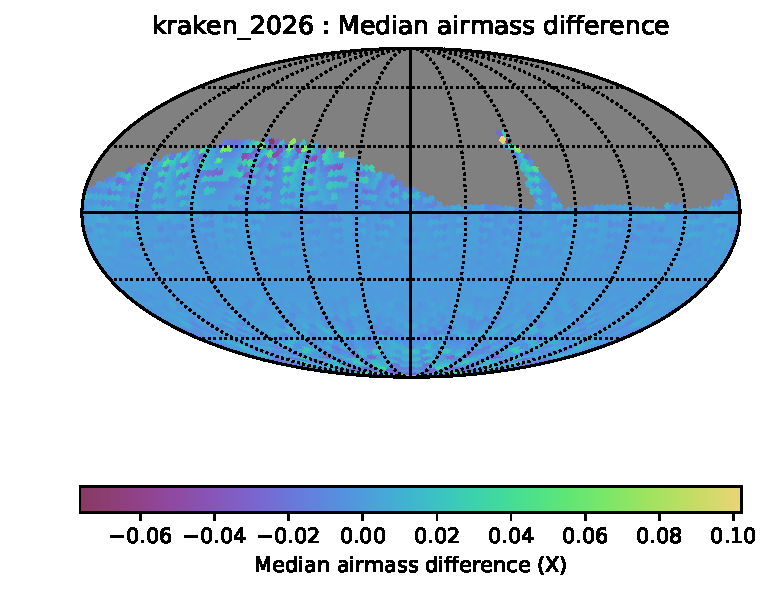
\includegraphics[width=0.49\textwidth]{figures/kraken_2026_Median_airmass_difference_HEAL_SkyMap.pdf}
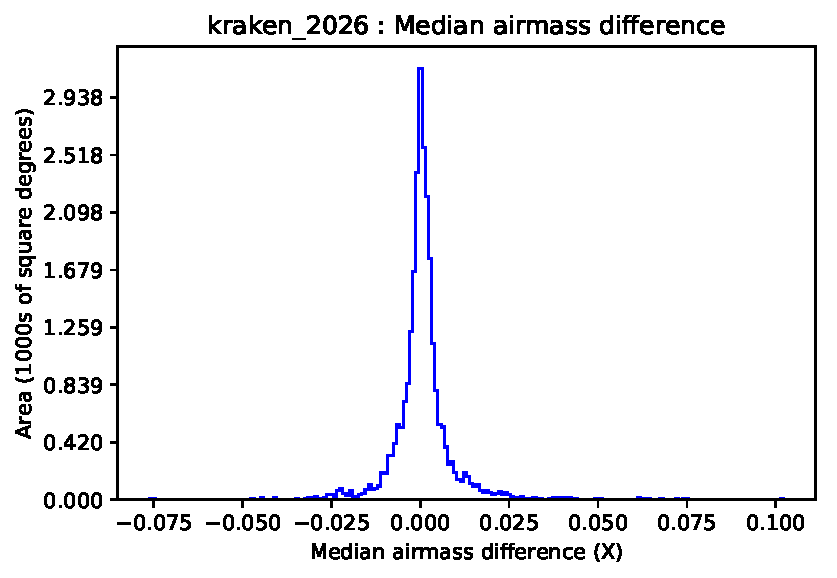
\includegraphics[width=0.49\textwidth]{figures/kraken_2026_Median_airmass_difference_HEAL_Histogram.pdf}
%\vskip -1.3in
\caption{The median airmass difference  in all bands across the sky for simulated survey
kraken\_2026 is shown in the left panel. The HealPix histogram of the median airmass differences
across the sky is shown in the right panel.}
\label{fig:airmass_diff}
\end{figure}

\section{Comparison of slew times and number of visits}

There are not many major changes to the overall behavior and performance of the new simulations
relative to baseline2018. The largest effect is seen in the slew time distributions (see Figure \ref{fig:slew_diff}) and statistics summarized in
Table \ref{tab:slewtime-comparison}. This comparison shows that by enabling a crawling dome, the mean
slew time decreases by 15 $\%$, and the median slew time decreases by 17 $\%$, relative to baseline2018a.
The shorter median and mean slew times have the added benefit of increasing the total number of
observations of the course of the entire survey. Including dome crawl increases the total number of visits in
pontus\_2003 by 3 $\%$, relative to baseline2018a. Including the longer CL delay in kraken\_2026, in addition to
dome crawl, results in 3,539 fewer visits relative to pontus\_2003, which is only a loss of $0.1\%$ over course of the
entire survey. For the reminder of this document we will focus on the comparison of kraken\_2026
to baseline2018a, and the overall details of kraken\_2026. The discussion of pontus\_2003 up to this point was to
illustrate the benefit of the dome crawl in isolation, but the inclusion of the longer CL correction in kraken\_2026 is
more realistic given it a hardware constraint rather than tunable characteristic of the survey.

\begin{table}[htp]
\caption{Comparison of slew time statistics between baseline2018a and the new simulations with dome crawl.}
\begin{center}
\small
\begin{tabular}{lrrr}
\toprule
{}                                         &   baseline2018a  &   pontus\_2003  &  kraken\_2026 \\
 Mean slewTime All visits    &           7.92          &         6.74          & 6.79               \\
 Median slewTime All visits &          5.18           &        4.79           & 4.79               \\
 Min slewTime All visits       &           2               &         2               & 2                     \\
 Max slewTime All visits      &         143             &       140             & 156                 \\

\bottomrule
\end{tabular}
\end{center}
\label{tab:slewtime-comparison}
\end{table}

\begin{figure}[ht]
\centering
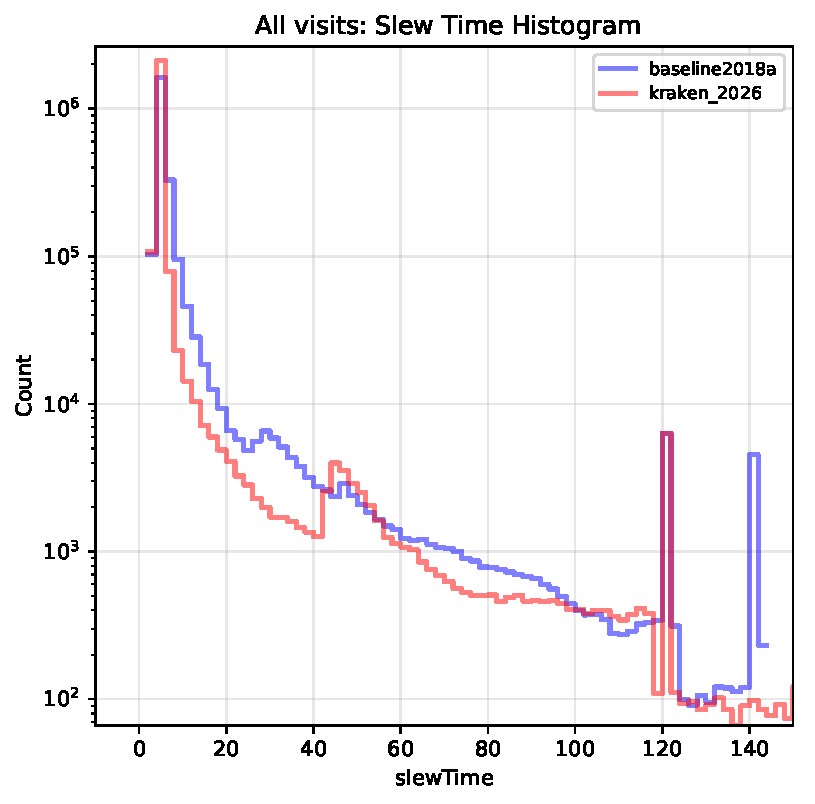
\includegraphics[width=0.49\textwidth]{figures/kraken_2026_baseline2018a_Slew_Time_Histogram_All_visits_ONED_ComboBinnedData.pdf}
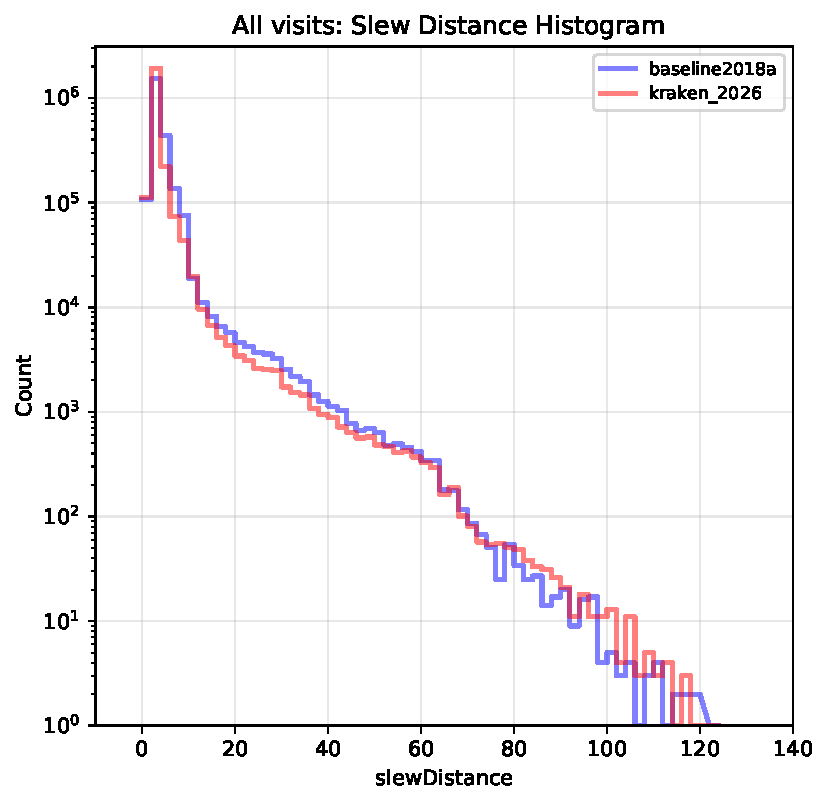
\includegraphics[width=0.49\textwidth]{figures/kraken_2026_baseline2018a_Slew_Distance_Histogram_All_visits_ONED_ComboBinnedData.pdf}
%\vskip -1.3in
\caption{The slew time histograms for baseline2018a and kraken\_2026 are shown in the left panel and
the slew distance histograms are shown in the right panel.}
\label{fig:slew_diff}
\end{figure}

\begin{table}[htp]
\caption{Comparison of NVisits statistics between baseline2018a and the new simulations with dome crawl.}
\begin{center}
\small
\begin{tabular}{lrrr}
\toprule
{}                                        &   baseline2018a  &   pontus\_2003     &  kraken\_2026   \\
Nvisits All props                 &     2,372,700       &     2,441,927         &    2,438,388       \\
Median Nvisits per night.   &         785             &         808               &      806               \\
\bottomrule
\end{tabular}
\end{center}
\label{tab:nvisits-comparison}
\end{table}

 \section{New baseline survey recommendation}
 \subsection{Comparison of kraken\_2026 to baseline2018a}

The SRD metrics for kraken\_2026 and baseline2018a are shown in Table~\ref{tab:srd-comparison}.
The FO metric evaluates the overall efficiency of observing. foNv: out of 18000.00 sq degrees, the area receives at least X and
a median of Y visits (out of 825, if compared to benchmark). fOArea: this many sq deg (out of 18000.00 sq deg if compared to benchmark)
receives at least 825 visits. From the comparison in Table~\ref{tab:srd-comparison}, we see that baseline2018a and kraken\_2026 perform
at a very similar level across the SRD metrics. The largest improvements in kraken\_2026 are in the fONv number of visits and
the Rapid Revisit Area in the WFD. In Table~\ref{tab:baseline_comparison} we compare other select metrics in baseline2018a
and kraken\_2026.

\begin{table}[htp]
\caption{Comparison of SRD metrics between kraken\_2026 and baseline2018a.}
\begin{center}
\small
\begin{tabular}{lrr}
\toprule
{}                                                                                       &   baseline2018a &   kraken\_2026 \\
\midrule
 fOArea fO WFD                                           &       18040.6       &     18040.6   \\
 fOArea/benchmark fO WFD                        &           1.002       &         1.002 \\
 fONv MedianNvis fO WFD                          &         912            &       938     \\
 fONv MinNvis fO WFD                                &         835            &       857     \\
 fONv/benchmark MedianNvis fO WFD       &           1.105       &         1.137 \\
 fONv/benchmark MinNvis fO WFD             &           1.012       &         1.039 \\
 Median Parallax Error @ 22.4 WFD                               &           1.638       &         1.606 \\
 Median Parallax Error @ 24.0 WFD                               &           6.32         &        6.175 \\
 Median Proper Motion Error @ 20.5 WFD                     &          0.169        &        0.166 \\
 Median Proper Motion Error @ 24.0 WFD                     &           1.713       &         1.677 \\
  Area (sq deg) RapidRevisits WFD                                &     9192.91        &       10757.1 \\
\bottomrule
\end{tabular}
\end{center}
\label{tab:srd-comparison}
\end{table}

\begin{table}
\caption{Comparison of select metrics between baseline2018a and kraken\_2026.}
\small
\begin{tabular}{lrr}
\toprule
{}                                                     &   baseline2018a &   kraken\_2026 \\
\midrule
Nvisits All props                          &     2,372,700   &  2,438,388       \\
Mean NVisits Per night OneDSlicer          &        784.36     &         806.08 \\
Fraction of total NVisits WFD              &            0.86 &          0.86 \\
Normalized Teff all bands                  &            0.56 &          0.56 \\
Median NVisits WFD u band HealpixSlicer    &              62 &            64 \\
Median NVisits WFD g band HealpixSlicer    &              87 &            90 \\
Median NVisits WFD r band HealpixSlicer    &             200 &           206 \\
Median NVisits WFD i band HealpixSlicer    &             199 &           204 \\
Median NVisits WFD z band HealpixSlicer    &             183 &           186 \\
Median NVisits WFD y band HealpixSlicer    &             182 &           188 \\
Median NVisits WFD all bands HealpixSlicer &             912 &           938 \\
Median CoaddM5 WFD u band HealpixSlicer    &          25.615 &        25.651 \\
Median CoaddM5 WFD g band HealpixSlicer    &          27.11  &        27.149 \\
Median CoaddM5 WFD r band HealpixSlicer    &          27.188 &        27.201 \\
Median CoaddM5 WFD i band HealpixSlicer    &          26.613 &        26.618 \\
Median CoaddM5 WFD z band HealpixSlicer    &          25.707 &        25.72  \\
Median CoaddM5 WFD y band HealpixSlicer    &          24.892 &        24.906 \\
Median Fraction of visits in pairs (15-60 min) gri WFD+NES HealpixSlicer &  0.901 &         0.876 \\
Median Inter-Night Gap WFD all bands (per healpix)            &           1.96  &          1.96 \\
Median seeingEff WFD r band                &           0.849  &         0.854 \\
Median slewTime All visits                 &           5.18   &         4.79 \\
Total Filter Changes All visits            &          10644   &         10813     \\
Median Normalized Airmass all bands        &          1.01    &         1.01  \\
Open Shutter Fraction                      &          0.716   &         0.735 \\
\bottomrule
\end{tabular}
\label{tab:baseline_comparison}
\end{table}

\subsection{Details of kraken\_2026}

The proposed new baseline simulated survey, kraken\_2026, has the following basic properties:

\begin{enumerate}
\item The total number of visits is 2,438,388, with 86.0\% spent on
the main Wide, Fast, Deep (WFD) survey, 5.0\% on the
North Ecliptic Spur proposal, 1.6\% on the Galactic Plane proposal, 2.0\%
on the South Celestial Pole proposal, and 5.0\% on the Deep Drilling
Cosmology proposal (5 fields).\footnote{The community-contributed white papers leading to the
Deep Drilling fields defined in the Baseline Cadence can be found via
\url{https://community.lsst.org/t/deep-drilling-whitepapers/732}.}

\item The median number of visits per night is 806, the range is
144 to 1093, with 3,025 observing nights. The mean slew time is 6.79
seconds (median: 4.79 sec) and the total exposure time (after 10 years) is 73.2 Msec (total number of visits $\times$ mean exposure time).
The surveying efficiency, or the median total open shutter time (per night)
as a fraction of the observing time (the ratio of the open shutter time to
the sum of the open shutter time, readout time and slew time) is 74\%.

\item The mean number of filter changes per night 3.18. The total number of filter changes through the survey is 10,813.

\item In the $r$ band, the median effective seeing for all proposals is 0.87 arcseconds.
The median airmass of all visits, for all filters and all proposals is 0.89.
The median single-visit $5\sigma$ depth for point sources in $r$ band in the WFD area is 24.26 (using the best
current estimate of the fiducial depth at airmass of one, $m_5(r)=24.34$).
The variation of the median airmass and seeing for the $r$
band observations with the position on the sky is shown in
\autoref{fig:baseline_airmass}.

\item The median single-visit depths for WFD fields are (23.34, 24.65, 24.26,
23.69, 22.78, 22.00) in the $ugrizy$ bands.

\item The median number of visits per HealPix in the WFD in the $ugrizy$ bands is
(64, 90, 206, 204, 186,188), respectively. These medians exceed the requested
number of visits (design specification from the SRD\footnote{The LSST
Science Requirements Document (SRD) is available as
\url{http://ls.st/srd}}) of (56, 80, 184, 184, 160, 160) in the $ugrizy$
bands. The SRD values are quoted for OpSim fields, but the visits per HealPix
is a good approximation.

\item The median coadded $5\sigma$ depth
for point sources in the $ugrizy$ bands is (25.6, 27.1, 27.2, 26.6,
25.7, 24.9), respectively, for the WFD area. The distribution
of coadded depth across the sky is fairly uniform, as illustrated in \autoref{fig:baseline_coadd}.

\item Restricted to the WFD fields, a unique area of
18,000 square degrees received a minimum 857 and a median of 940 visits per field (summed over bands;
the SRD design value is 825).

\item The median trigonometric parallax and proper motion errors are
1.8 mas and 0.17 mas/yr, respectively, for bright sources (limited by
assumed systematic errors in relative astrometry of 10 mas), and 7.1
mas and 1.8 mas/yr for points sources with $r=24$ (assuming a flat
spectral energy distribution), in the WFD fields. The variation of parallax
and proper motion errors across the sky is visualized in \autoref{fig:baseline_parapm}.
\end{enumerate}

Here we only provide the basic
performance parameters of the special proposals.
The North Ecliptic Spur proposal (5.0\% of the observing time) obtained  a total of 132,644 in $griz$ bands.
These fields are placed along the northern part of the Ecliptic.
The Galactic Plane proposal (1.6\%) obtained 38,676 total visits in $ugrizy$
across the region extending in Galactic latitude 10 degrees
from the Galactic center, with the boundary approaching the Galactic
equator linearly with longitude, and the zone ending at $l=90$ deg.
and at $l=270$ deg.
The South Celestial Pole proposal (2.0\%) obtained
obtained 47,679 total visits in $ugrizy$, respectively, for fields centers with Dec $<-62.5$ deg.
The Deep Drilling proposal (5.0\%) included 5 fields, with each obtaining several thousand visits per band
as required for various cosmology investigations. The coadded $5\sigma$ depths for these fields are much
fainter than for the main survey: the median values are (27.9, 28.6, 28.7, 28.2, 27.8, 26.6) in the $ugrizy$ bands, respectively.


\section{Known issues}

The overall observing strategy in kraken\_2026 did not change relative to baseline2018a, so it still has issues listed in the
previous baseline document describing that baseline.

There is the new issue of the airmass values that are derived from HealPix simulated sky maps, and this will be addressed
in new versions of \opsim.

\section{Reproducibility of new baseline survey and its evaluation}

The kraken\_2026  simulated survey was produced using \opsim v4, v4.1.2.2.  This overarching package designation includes, specifically:
\begin{itemize}
\item Observatory model (ts\_observatory\_model) version 1.1
\item Astro sky model (ts\_astrosky\_model) version 1.1
\item Dateloc (ts\_dateloc) version 1.0
\item Sky brightness model (sims\_skybrightness\_pre) version 2.8.0.sims
\item Sky brightness precalculated file version 4f5efe2
\item M5 constants (sims\_utils) version 2.8.0.sims
\item SOCS (sims\_ocs) version 1.1.1
\item Scheduler (ts\_scheduler) version 1.2.2
\end{itemize}

The configuration parameters were left as the defaults for this version, with the exception that the airmass bonus was set to 0 for all proposals and the $HA$ bonus was set to 0.3, with $HA_{max}$ = 3 hrs
for all proposals except Deep Drilling, where it was $HA$ bonus = 0.3 and $HA_{max}$ = 6 hrs. The configuration also used the
crawling dome model, and the closed loop active optics delay was increased from 20 seconds to 36 seconds.
These two changes in configuration are the only difference between kraken\_2026 and baseline2018a.
The details of all configuration parameters can be found in the sqlite output database, in the Config table, as well as in the
github repo housing this document (\url{https://github.com/lsst-ts/opsim4_config/tree/baseline2018_dc_cl/config_run}).

The simulated survey output database for kraken\_2026 is available in the github repo housing this document, together with MAF analysis outputs.
These MAF outputs can also be found online at \url{http://astro-lsst-01.astro.washington.edu:8080}.

%%%%%%%%%

\clearpage
\clearpage

\begin{figure}[ht]
\centering
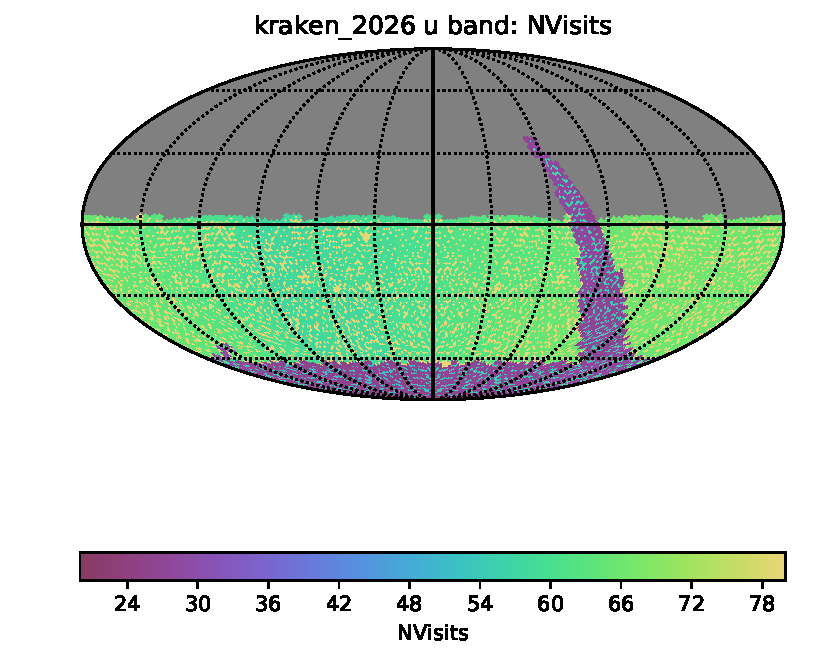
\includegraphics[width=0.43\textwidth]{figures/kraken_2026_NVisits_u_band_HEAL_SkyMap}
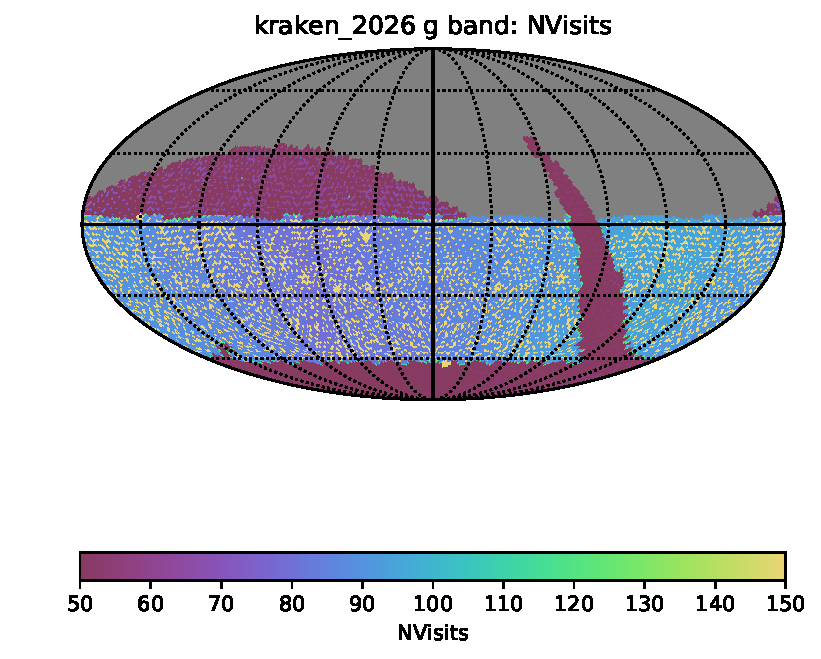
\includegraphics[width=0.43\textwidth]{figures/kraken_2026_NVisits_g_band_HEAL_SkyMap} \\
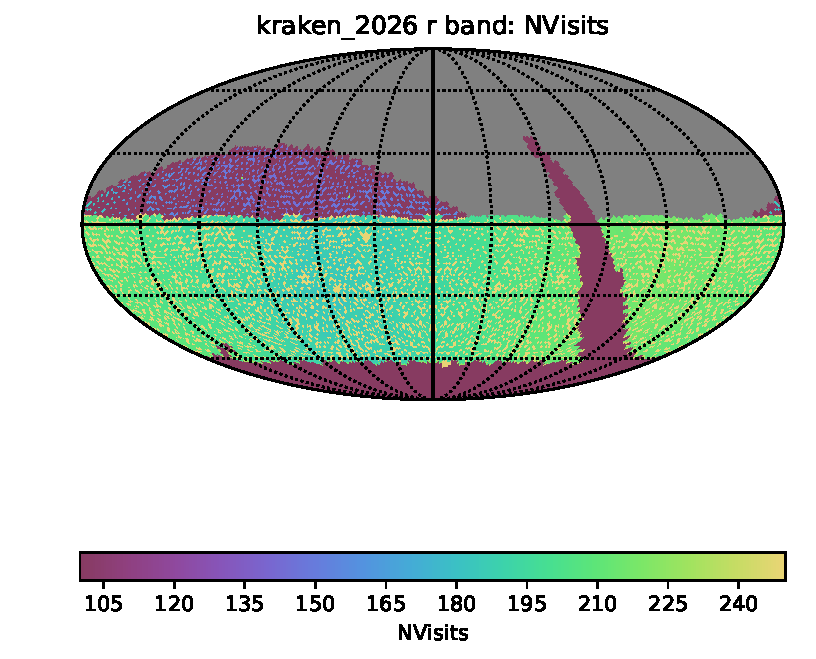
\includegraphics[width=0.43\textwidth]{figures/kraken_2026_NVisits_r_band_HEAL_SkyMap}
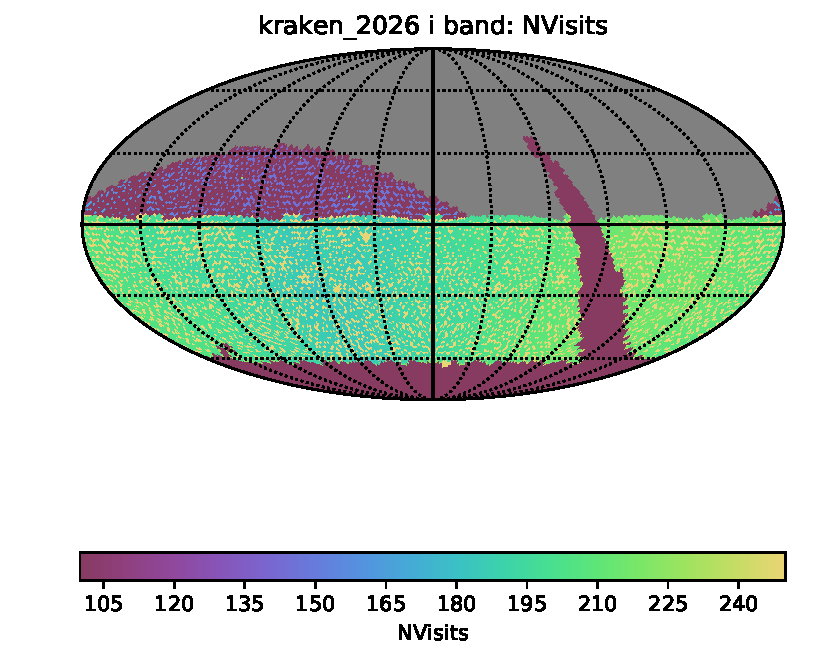
\includegraphics[width=0.43\textwidth]{figures/kraken_2026_NVisits_i_band_HEAL_SkyMap} \\
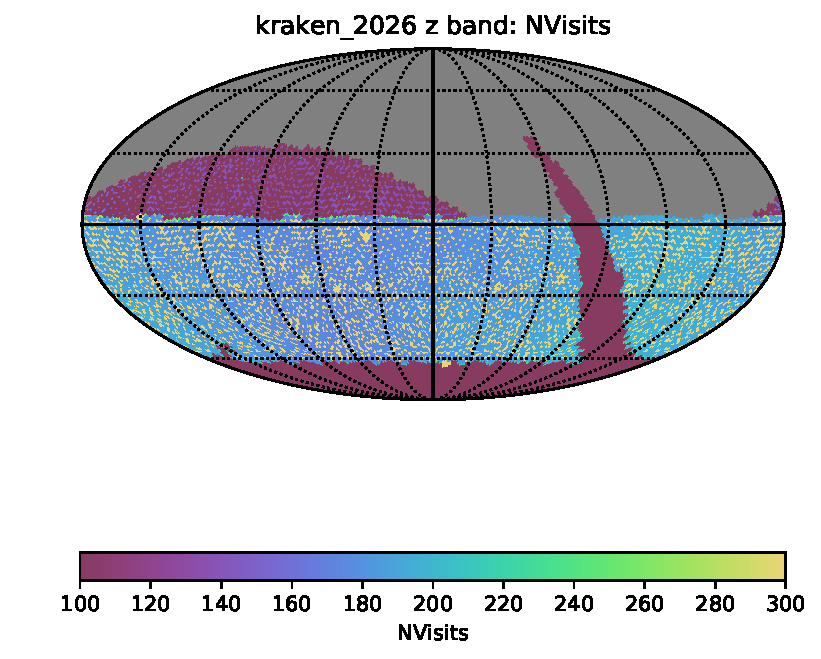
\includegraphics[width=0.43\textwidth]{figures/kraken_2026_NVisits_z_band_HEAL_SkyMap}
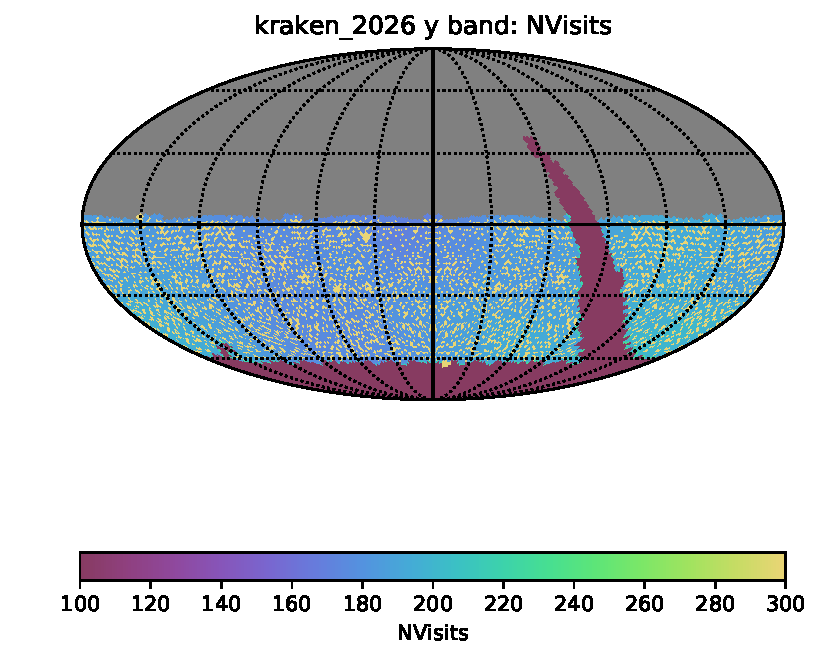
\includegraphics[width=0.43\textwidth]{figures/kraken_2026_NVisits_y_band_HEAL_SkyMap}
\caption{Number of visits per filter for kraken\_2026.
\label{fig:baseline_nvisits}}
\end{figure}

\begin{figure}[ht]
\centering
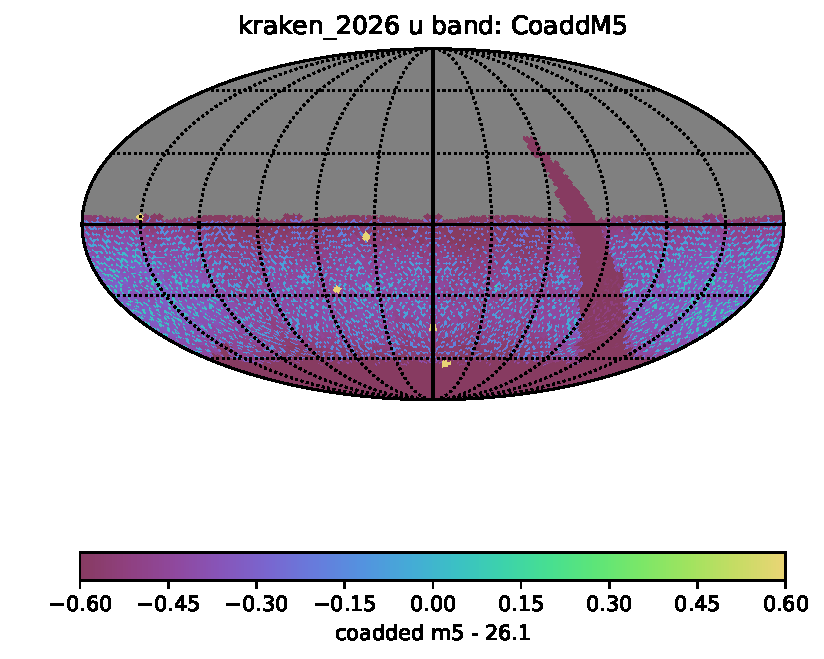
\includegraphics[width=0.43\textwidth]{figures/kraken_2026_CoaddM5_u_band_HEAL_SkyMap}
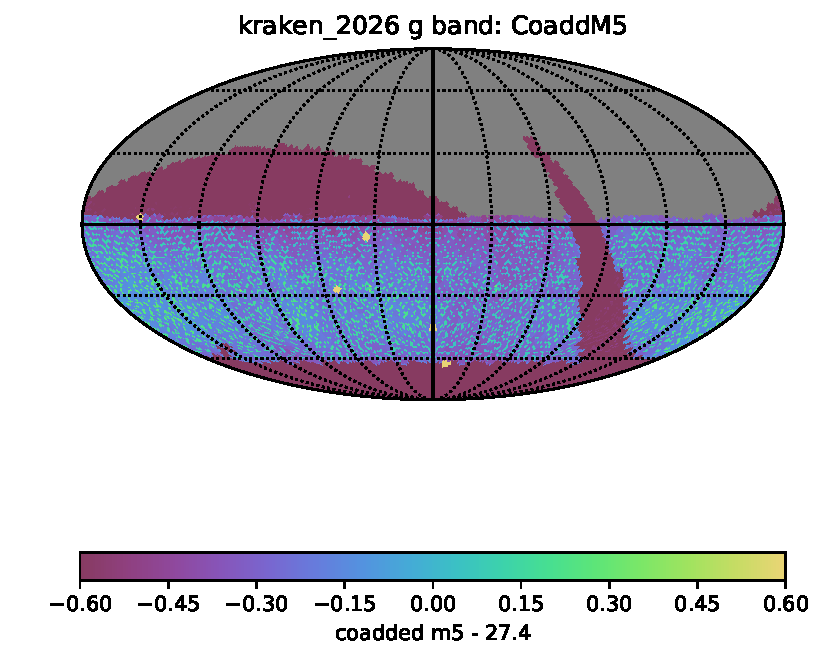
\includegraphics[width=0.43\textwidth]{figures/kraken_2026_CoaddM5_g_band_HEAL_SkyMap} \\
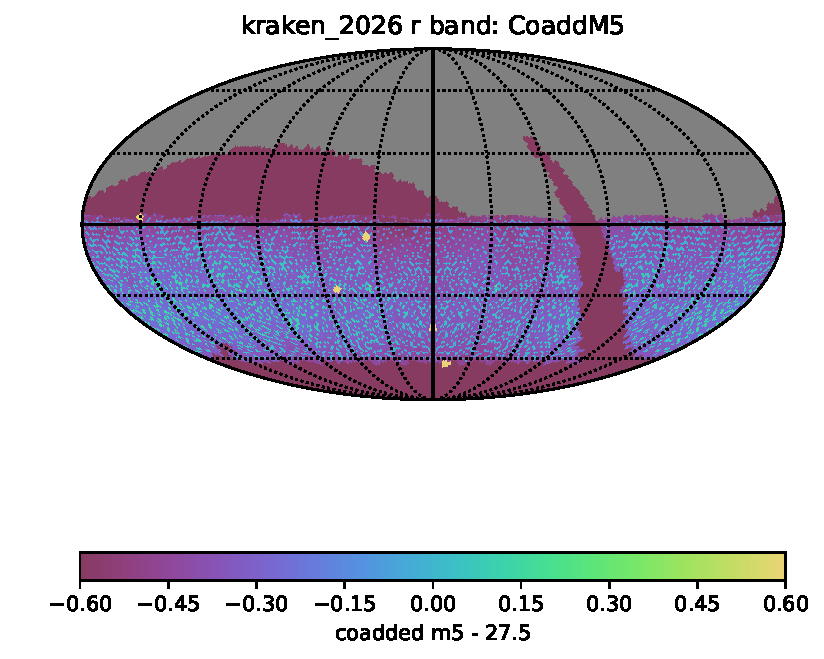
\includegraphics[width=0.43\textwidth]{figures/kraken_2026_CoaddM5_r_band_HEAL_SkyMap}
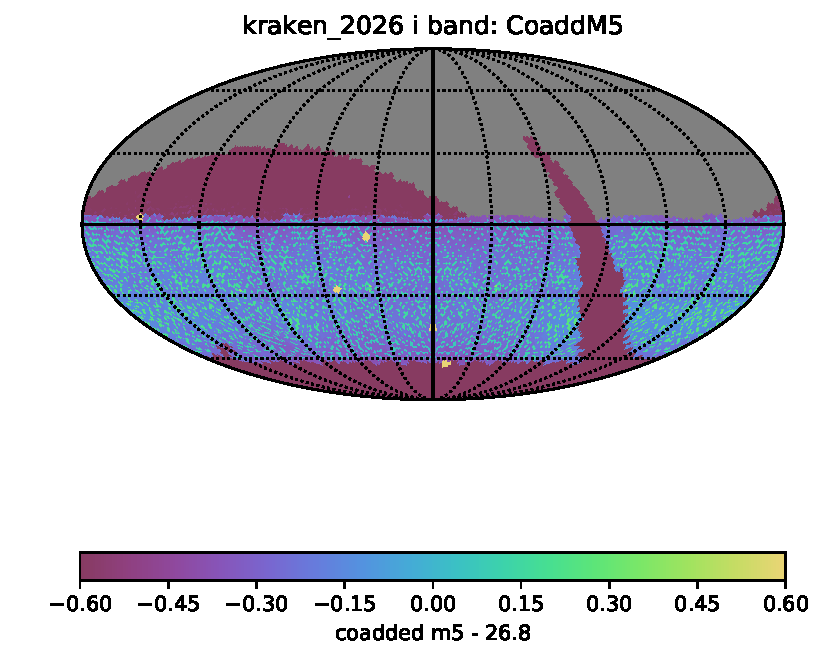
\includegraphics[width=0.43\textwidth]{figures/kraken_2026_CoaddM5_i_band_HEAL_SkyMap}  \\
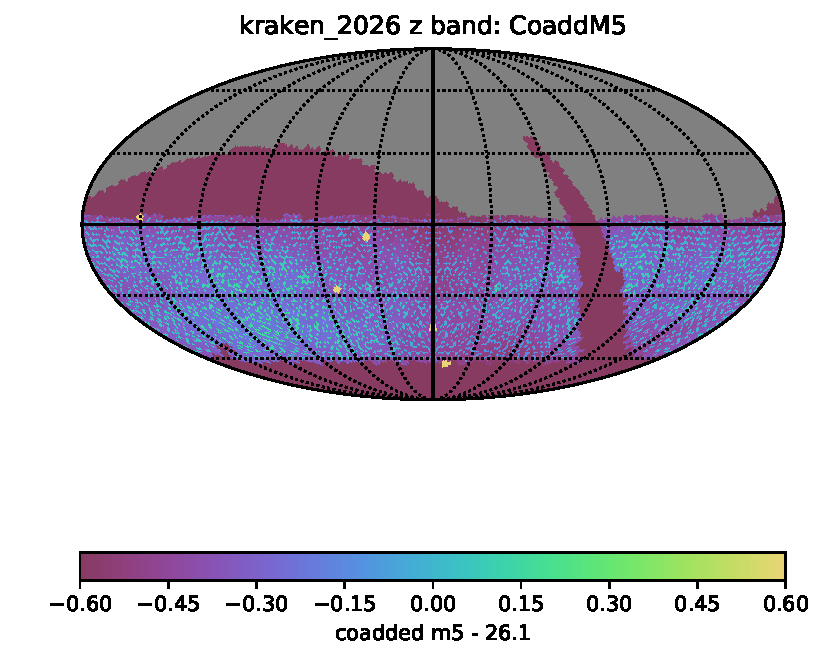
\includegraphics[width=0.43\textwidth]{figures/kraken_2026_CoaddM5_z_band_HEAL_SkyMap}
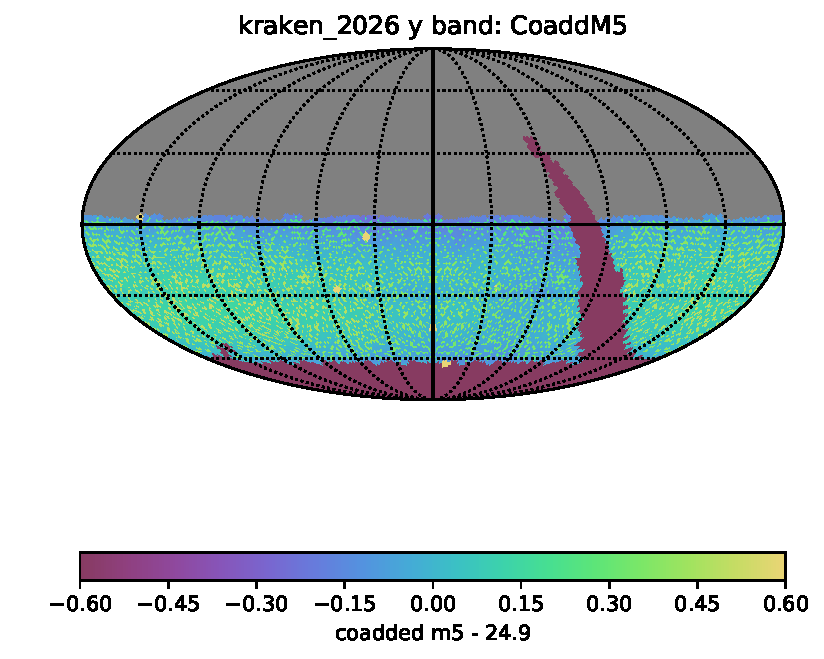
\includegraphics[width=0.43\textwidth]{figures/kraken_2026_CoaddM5_y_band_HEAL_SkyMap}
\caption{Coadded depth per filter for kraken\_2026. In each band, the nominal coadded depth expected if
visits were allocated between bands as suggested in the SRD and obtained individual image $5\sigma$ depths
as expected. More positive numbers indicate fainter coadded depths. The small dots visible in each band correspond
to the deep drilling fields.
\label{fig:baseline_coadd}}
\end{figure}

\begin{figure}[ht]
\centering
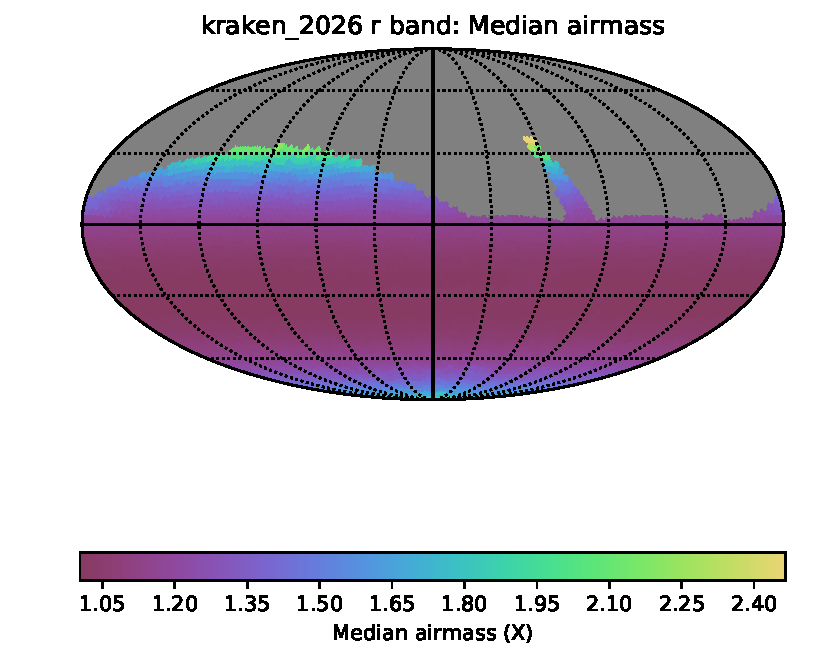
\includegraphics[width=0.49\textwidth]{figures/kraken_2026_Median_airmass_r_band_HEAL_SkyMap}
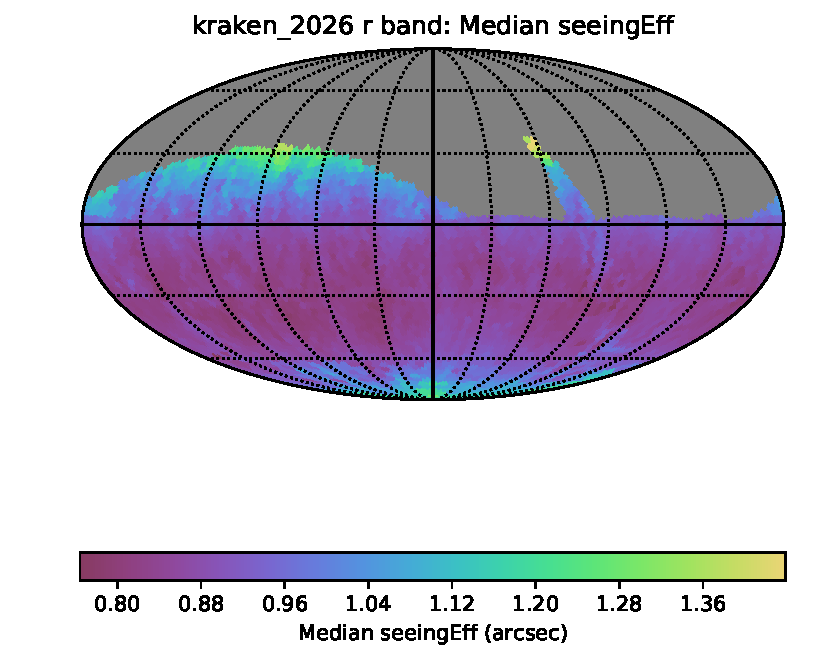
\includegraphics[width=0.49\textwidth]{figures/kraken_2026_Median_seeingEff_r_band_HEAL_SkyMap}
%\vskip -1.3in
\caption{The median airmass in the $r$ band across the sky for simulated survey
kraken\_2026 is shown in the left panel. For the main survey area, the maximum
allowed airmass was set to 1.5. The median seeingFWHMeff in the $r$ band across the sky
for simulated survey kraken\_2026 is shown in the right panel.}
\label{fig:baseline_airmass}
\end{figure}


\begin{figure}[htb]
\centering
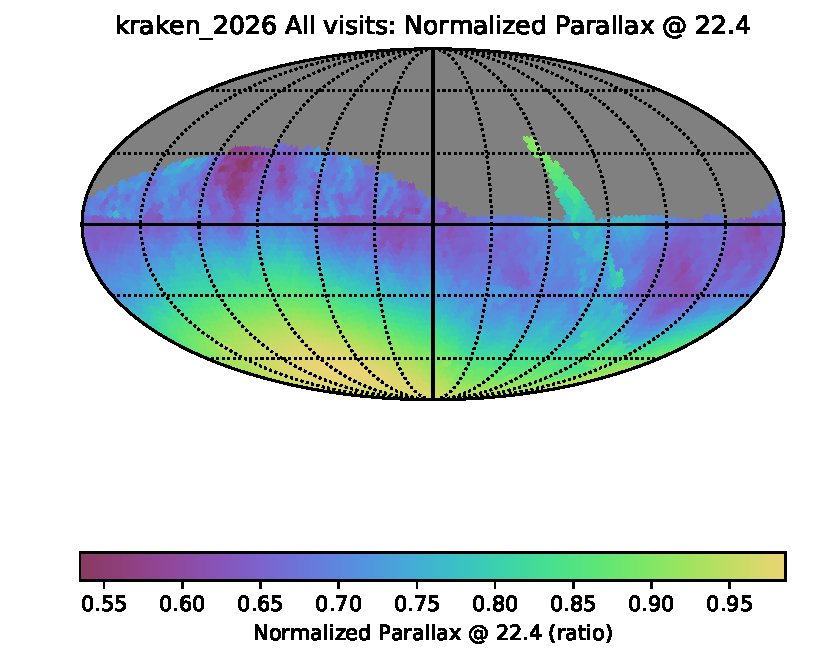
\includegraphics[height=2.4in]{figures/kraken_2026_Normalized_Parallax_@_22_4_All_visits_HEAL_SkyMap}
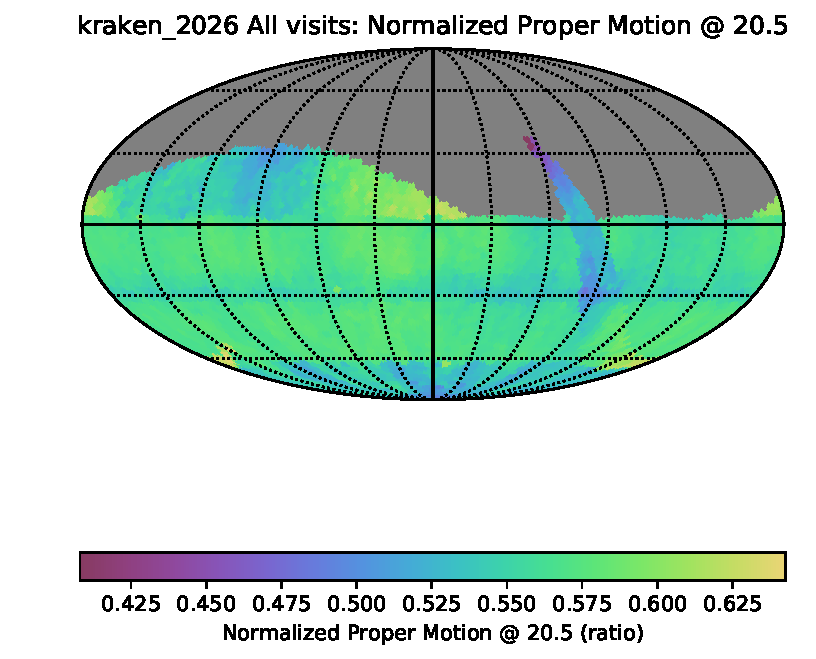
\includegraphics[height=2.4in]{figures/kraken_2026_Normalized_Proper_Motion_@_20_5_All_visits_HEAL_SkyMap} \\
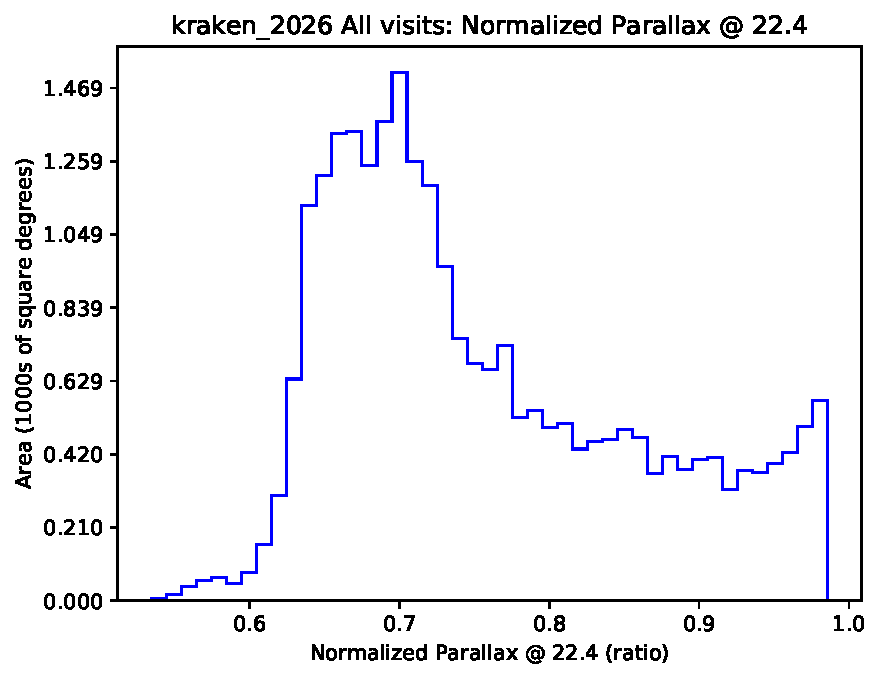
\includegraphics[height=2.2in]{figures/kraken_2026_Normalized_Parallax_@_22_4_All_visits_HEAL_Histogram}
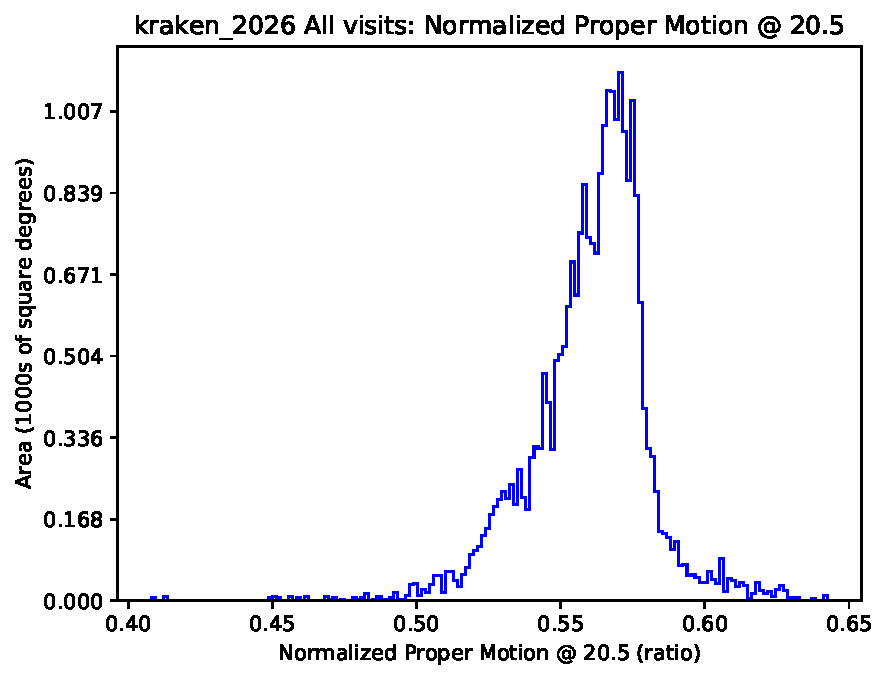
\includegraphics[height=2.2in]{figures/kraken_2026_Normalized_Proper_Motion_@_20_5_All_visits_HEAL_Histogram}
\caption{The trigonometric parallax errors (left) and proper motion errors (right), normalized
by the values for idealized perfectly optimized cadences (parallax: all the observations are taken
at maximum parallax factor, resulting in a peak at the South Ecliptic pole; proper motion:
a half of all visits are obtained on the first day and the rest on the last day of the survey). These normalized values are shown as
obtained for simulated survey kraken\_2026. Values closer to 1 indicate more optimal scheduling.
\label{fig:baseline_parapm}}
\end{figure}


\begin{figure}[htb]
\centering
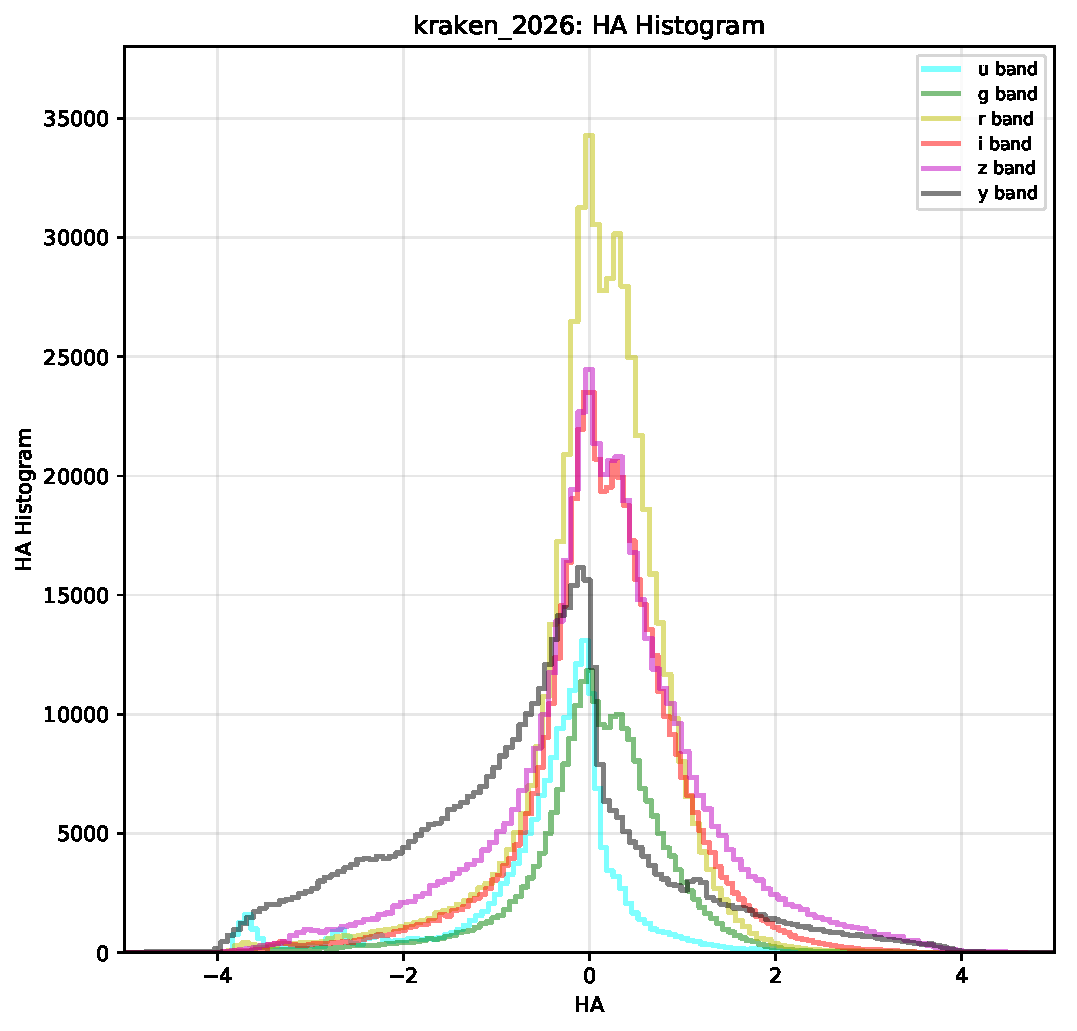
\includegraphics[height=2.4in]{figures/kraken_2026_HA_Histogram-ha_hist_per_filter.pdf}
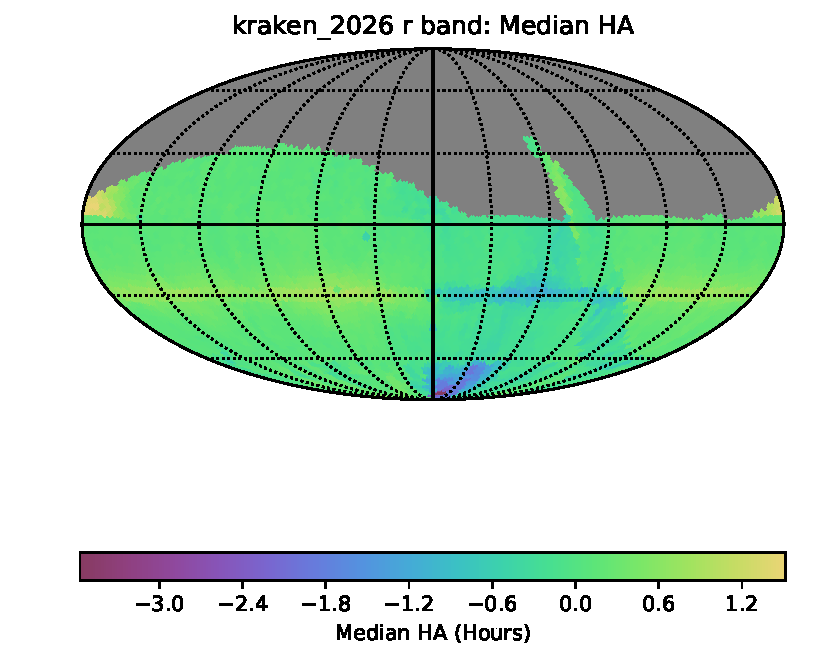
\includegraphics[height=2.4in]{figures/kraken_2026_Median_HA_r_band_HEAL_SkyMap.pdf}
\caption{Histograms in the left panel show the distribution of hour angles (HA) in
6 bands for all proposals from simulated survey kraken\_2026.
The right panel shows the distribution across the sky of the mean HA for
all observations in the $r$ band.
\label{fig:baseline_ha}}
\end{figure}


\begin{figure}[htb]
\centering
\vskip -0.0in
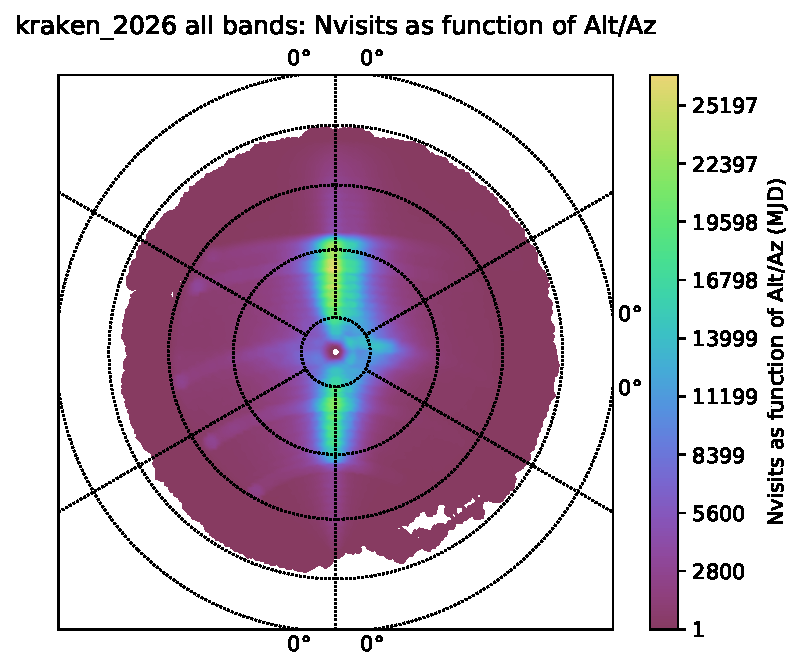
\includegraphics[height=2.5in]{figures/kraken_2026_Nvisits_as_function_of_Alt_Az_all_bands_HEAL_SkyMap.pdf}
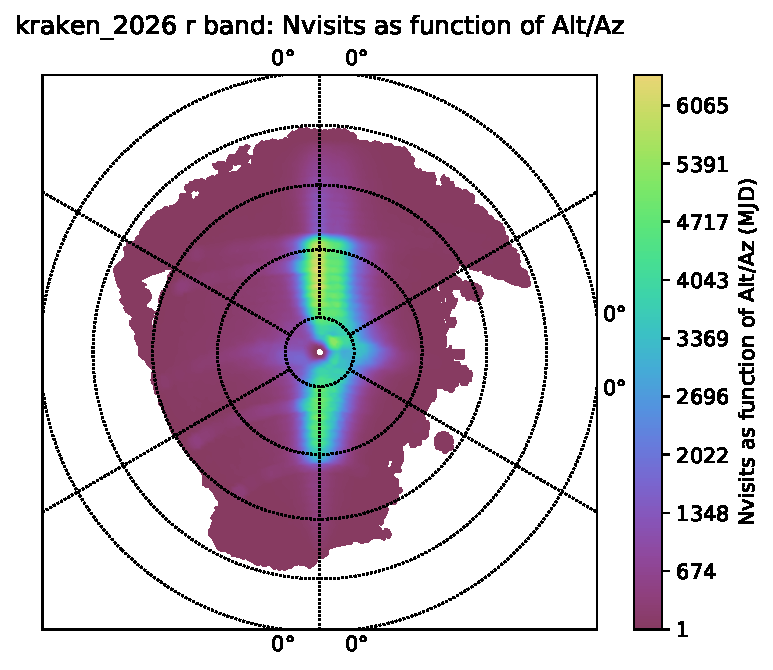
\includegraphics[height=2.5in]{figures/kraken_2026_Nvisits_as_function_of_Alt_Az_r_band_HEAL_SkyMap.pdf}
\vskip -0.1in
\caption{The color-coded map in the left panel shows the visit count from the
simulated survey kraken\_2026 in alt/az, using an equal-area Lambert projection,
with north on top and west towards the right, for all six bands and proposals
(Wide, Fast, Deep, Galactic Plane, Deep Drilling fields, North Ecliptic Spur, and South Celestial Pole region).
The right panel is analogous, but only shows the $r$ band visits.}
\label{fig:baseline_AltAz}
\end{figure}

\begin{figure}[htb]
\centering
\vskip -0.0in
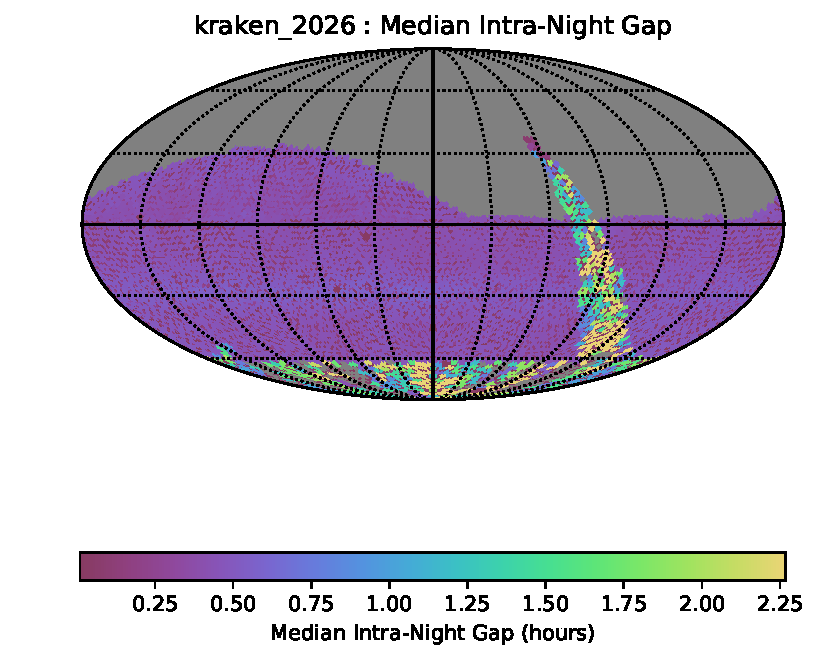
\includegraphics[height=2.3in]{figures/kraken_2026_Median_Intra-Night_Gap_HEAL_SkyMap.pdf}
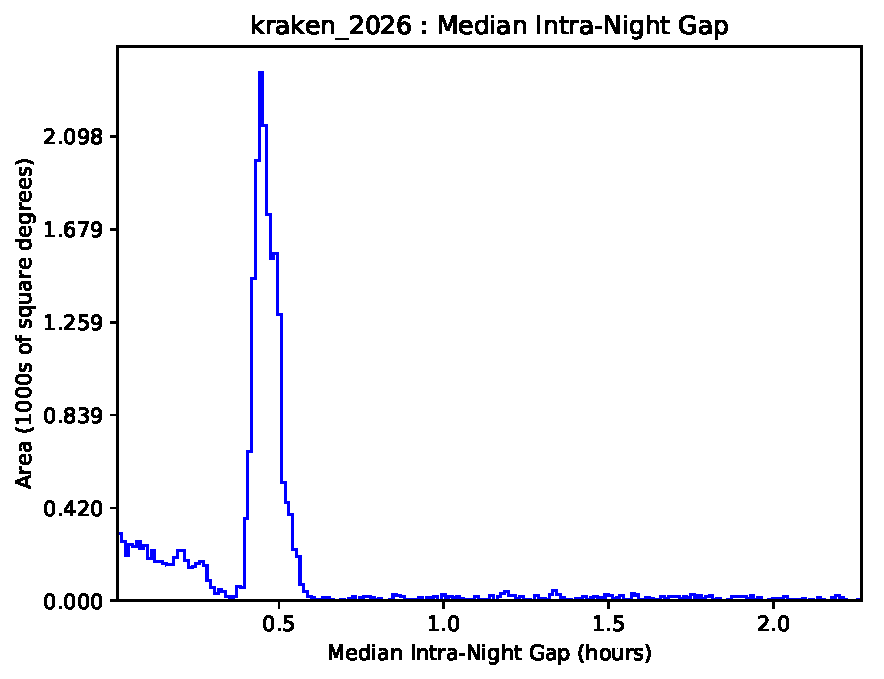
\includegraphics[height=2.3in]{figures/kraken_2026_Median_Intra-Night_Gap_HEAL_Histogram.pdf}
\vskip -0.1in
\caption{The median intra-night gap (or revisit time) for all proposals and all filters for  kraken\_2026.
The median gap between observations, when a field is observed multiple times in a night, is 27 minutes.
\label{fig:baseline_InterGapAll}}
\end{figure}


\begin{figure}[htb]
\centering
\vskip -0.0in
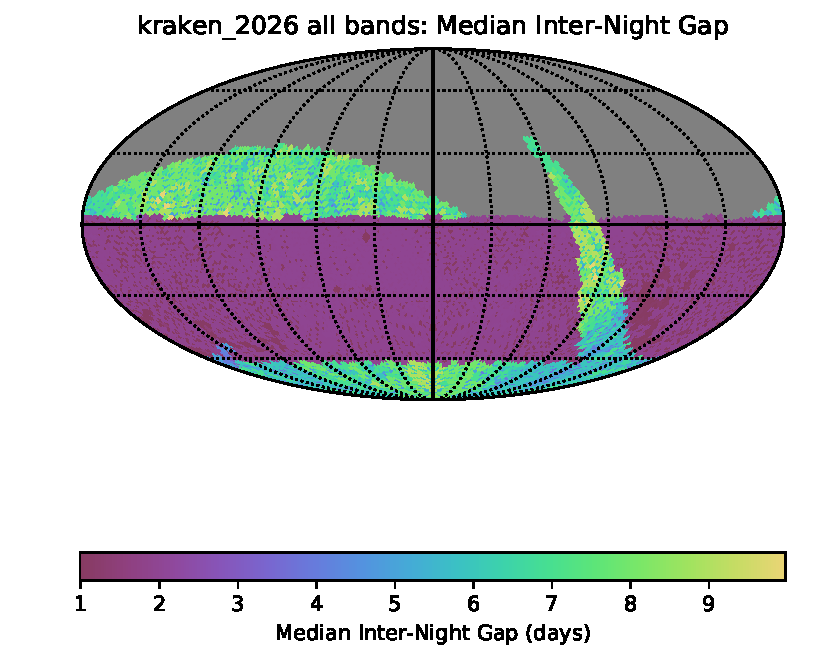
\includegraphics[height=2.3in]{figures/kraken_2026_Median_Inter-Night_Gap_all_bands_HEAL_SkyMap.pdf}
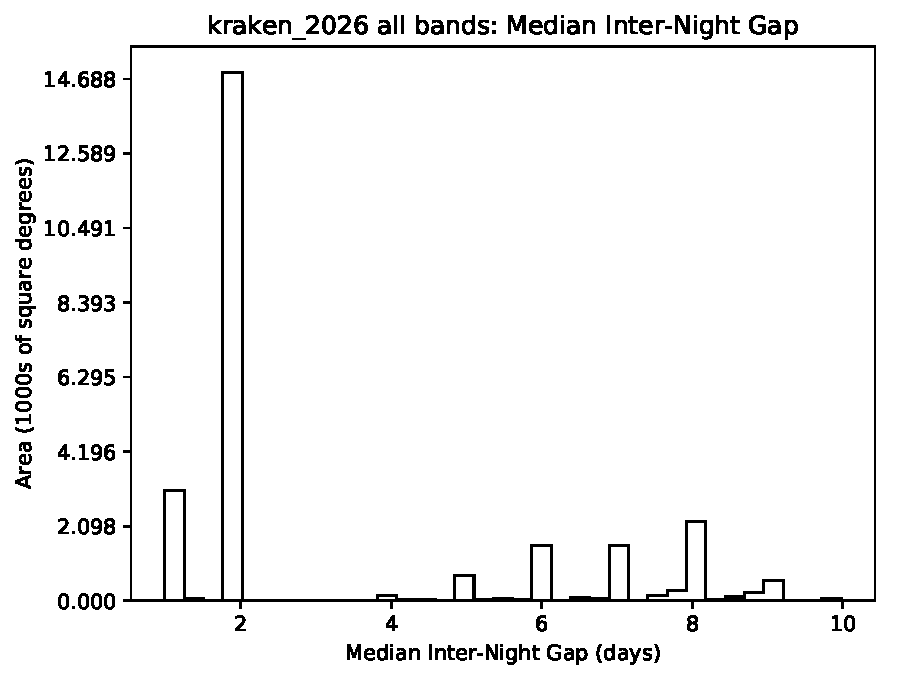
\includegraphics[height=2.3in]{figures/kraken_2026_Median_Inter-Night_Gap_all_bands_HEAL_Histogram.pdf}
\vskip -0.1in
\caption{The median inter-night gap (or revisit time)  for all proposals and all filters for kraken\_2026.
The median gap between nights with observations is 2 nights.
\label{fig:baseline_GapAll}}
\end{figure}


\begin{figure}[htb]
\centering
\vskip -0.0in
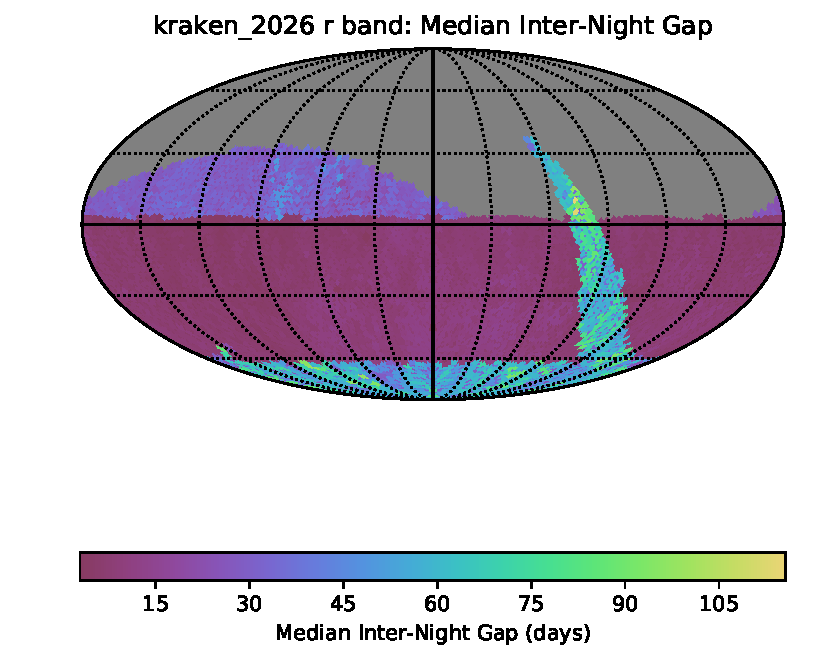
\includegraphics[height=2.3in]{figures/kraken_2026_Median_Inter-Night_Gap_r_band_HEAL_SkyMap.pdf}
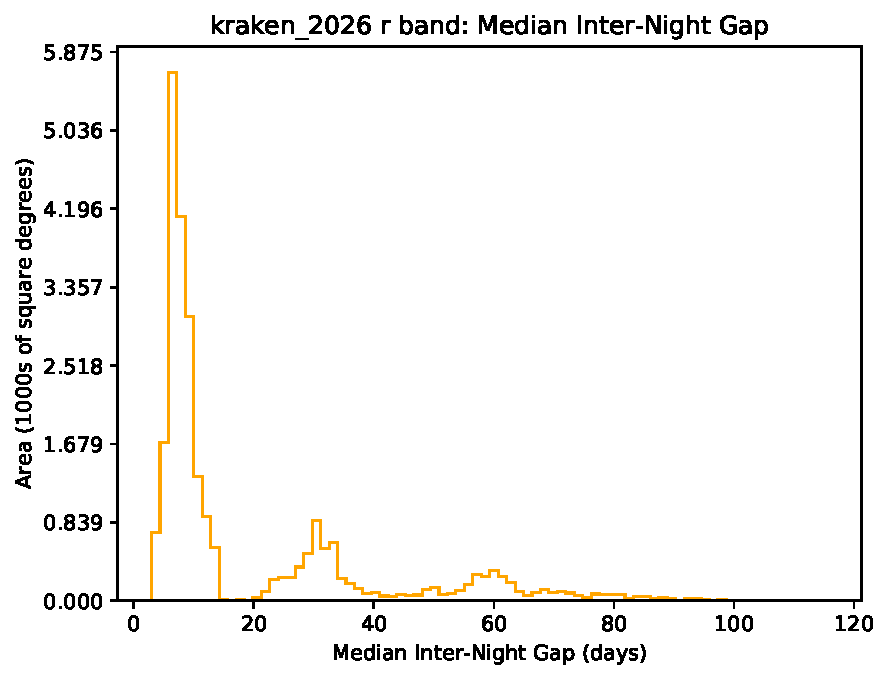
\includegraphics[height=2.3in]{figures/kraken_2026_Median_Inter-Night_Gap_r_band_HEAL_Histogram.pdf}
\vskip -0.1in
\caption{The median inter-night gap for $r$ band visits for all proposals for kraken\_2026.
On average, fields in the main survey get revisited in the $r$ band about every two weeks.}
\label{fig:baseline_Gapr}
\end{figure}


\begin{figure}[htb]
\centering
\vskip -0.0in
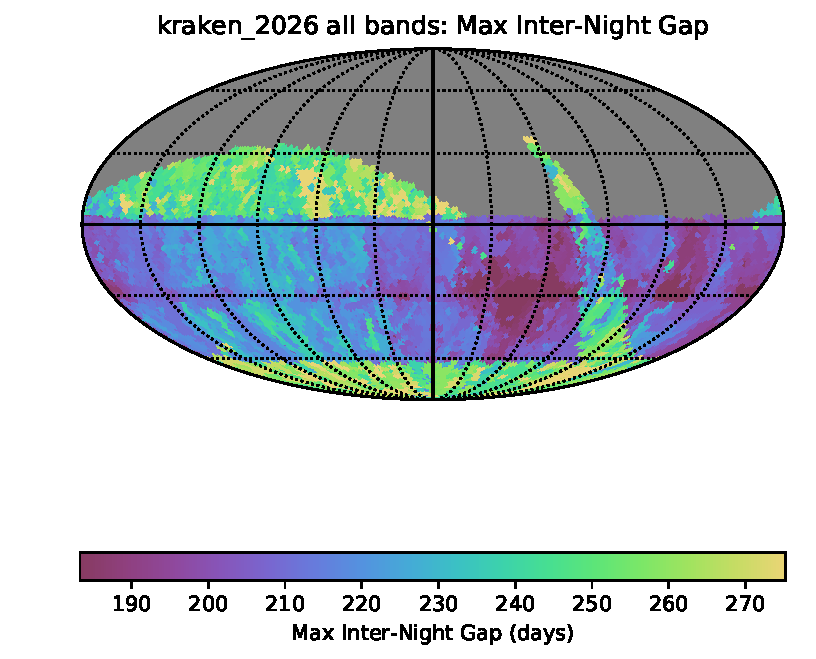
\includegraphics[height=2.3in]{figures/kraken_2026_Max_Inter-Night_Gap_all_bands_HEAL_SkyMap.pdf}
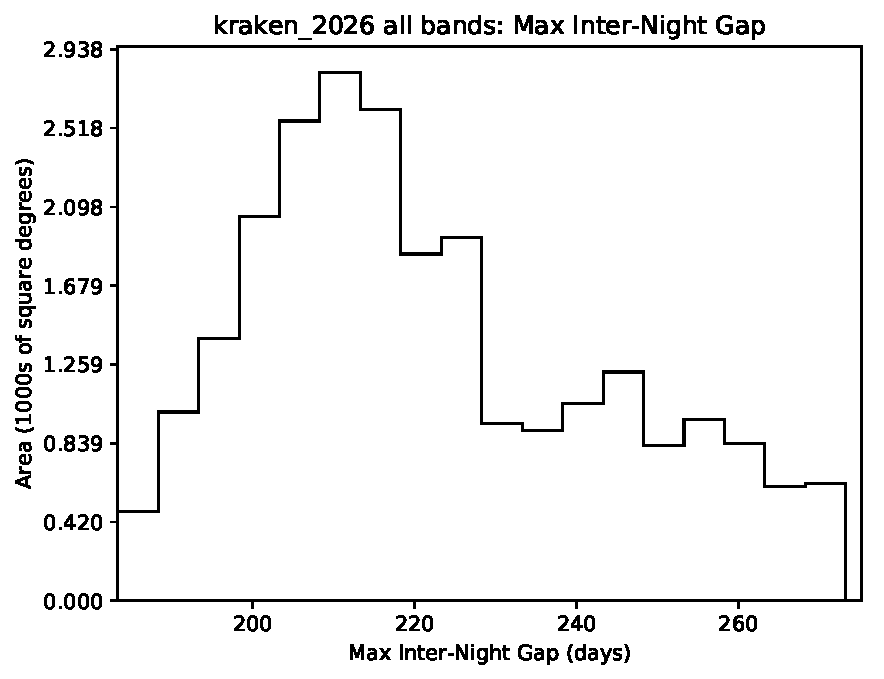
\includegraphics[height=2.3in]{figures/kraken_2026_Max_Inter-Night_Gap_all_bands_HEAL_Histogram.pdf}
\vskip -0.1in
\caption{The maximum inter-night gap (or revisit time) for all proposals and all filters for kraken\_2026.}
\label{fig:baseline_MAXGapAll}
\end{figure}



% Include all the relevant bib files.
% https://lsst-texmf.lsst.io/lsstdoc.html#bibliographies
% Set up the LSST texmf package to get these bibtex files.
%\bibliography{lsst,lsst-dm,refs_ads,refs,books}

\end{document}
